\chapter{The quasi-local approach: trapping horizons}
\label{s:loc}

\minitoc

\section{Introduction}

This chapter is in a draft stage.

\section{Trapped surfaces and singularity theorems}

\subsection{Trapped surfaces}

The concept of trapped surfaces has been introduced in Sec.~\ref{s:neh:trapped_surfaces}
(see in particular Fig.~\ref{f:neh:trapped_surf}). Let us recall that
a submanifold $\Sp$ of a $n$-dimensional spacetime ($n\ge 3$) is
a \defin{trapped surface}\index{trapped!surface} iff (i) $\Sp$ is a compact $(n-2)$-dimensional manifold
(without boundary), (ii) $\Sp$ is spacelike (positive definite induced metric)
and the two systems of null geodesics emerging orthogonally from $\Sp$ towards the future
locally converge, i.e. they have negative expansions at $\Sp$:
$\theta_{(\wl)} < 0$ and $\theta_{(\w{k})} < 0$ [Eq.~(\ref{e:neh:def_trapped_surf})],
$\wl$ and $\w{k}$ being
future-directed vectors tangent to these geodesics.

\begin{figure}
\centerline{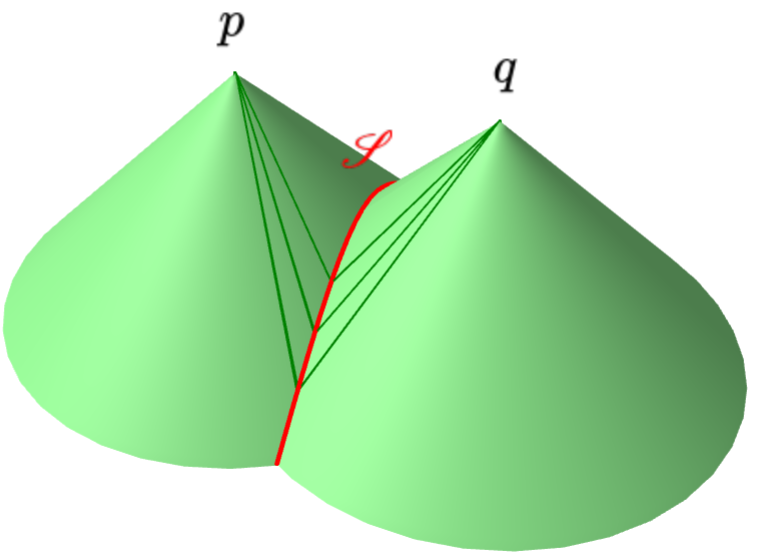
\includegraphics[width=0.6\textwidth]{loc_cone_intersect.png}}
\caption[]{\label{f:loc:cone_intersect} \footnotesize
Intersection $\Sp$ (red curve) of past light cones from two points $p$ and $q$ in Minkowski spacetime.
Some light rays emerging from $\Sp$ in the two orthogonal null directions are depicted; the two sets
of light rays are both converging. Yet $\Sp$ is not trapped because it is not compact.
\textsl{[Figure generated by the notebook \ref{s:sam:loc_cone_intersect}]}
}
\end{figure}



\begin{remark}
Trapped surfaces are sometimes called
\emph{closed trapped surfaces}\index{closed!trapped surface}\index{trapped!surface!closed --} (e.g. \cite{Penro65,HawkiE73}),
to stress their closed manifold aspect (compact without boundary).
We follow here the textbooks \cite{MisneTW73,Wald84} and call them merely
\emph{trapped surface}.
The closed aspect is a key piece of the definition, though. Without it, trapped surfaces would exist
in Minkowski spacetime, as shown by the intersection $\Sp$ of two past light cones. The surface $\Sp$
is spacelike (being a cross section of each light cone) and fulfils $\theta_{(\wl)} < 0$ and $\theta_{(\w{k})} < 0$. It fails to be a trapped surface for it is not compact. Truncating the light cones
would not help, because this would make $\Sp$ a manifold with boundary and hence not closed.
\end{remark}

%%%%%%%%%%%%%%%%%%%%%%%%%%%%%%%%%%%%%%%%%%%%%%%%%%%%%%%%%%%%%%%%%%%%%%%%%%%%%%%

\section{Trapping horizons}


